\documentclass[tikz,border=5mm]{standalone}
\usepackage{tikz-3dplot}

\begin{document}
\tdplotsetmaincoords{70}{110} % Set the 3D view angles

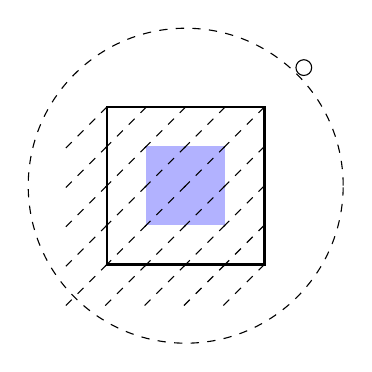
\begin{tikzpicture}[scale=1]
    % Draw the outer dashed circle
    \draw[dashed] (0,0) circle (2cm);

    % Draw the server rectangle
    \begin{scope}[canvas is xy plane at z=0]
        \draw[thick] (-1,-1) rectangle (1,1);
        % Add the solid rectangle on top
        \fill[blue!30] (-0.5,-0.5) rectangle (0.5,0.5);
    \end{scope}

    % Draw the small circle on the right corner
    \draw (1.5,1.5) circle (0.1cm);

    % Draw the vertical lines for 3D effect
    \foreach \x in {-1,-0.5,...,1}{
        \foreach \y in {-1,-0.5,...,1}{
            \draw[dashed,thin] (\x,\y) -- ++(0,0,1.5);
        }
    }

    % Draw the bottom edge of the server rectangle
    \draw[thick] (-1,-1) -- (1,-1);

    % Draw the back edge of the server rectangle
    \draw[thick] (1,-1) -- (1,1);

    % Draw the front edge of the server rectangle
    \draw[thick] (-1,1) -- (1,1);

    % Draw the left edge of the server rectangle
    \draw[thick] (-1,-1) -- (-1,1);
\end{tikzpicture}
\end{document}